\section{The Theory: Seven Propositions}
\label{sec:theory}

The theory is presented as seven numbered propositions with sub-propositions. Each sub-proposition is tagged: \textit{d} (definition), \textit{a} (postulate), \textit{t} (theorem), or \textit{o} (observation). Definitions are stipulative; postulates are assumed and falsifiable; theorems follow deductively from prior propositions; observations are empirical claims testable against the corpus. Table~\ref{tab:propositions} summarizes the seven main propositions and the formal apparatus each introduces. Propositions 1--4 are operationalized and tested against the corpus in Section~\ref{sec:empirical}. Propositions 5--7 introduce the agent, care, and multi-scale dynamics; they are formalized here, illustrated through worked examples in Section~\ref{sec:examples}, and yield falsifiable research programs in Section~\ref{sec:agenda}, but are not directly tested in the present study.

\subsection{Proposition 1: The world of form is all that is the case}
\label{sec:prop1}

The first proposition deliberately echoes the opening of Wittgenstein's \textit{Tractatus} \parencite{Wittgenstein1921}: where Wittgenstein begins with facts, the present theory begins with forms. The theory begins with ontology. An \textbf{object} is the simplest constituent of a form, indivisible within the chosen level of analysis. A \textbf{configuration} is an assembly of objects; form is the structure of the configuration. These two definitions fix the analytical substrate: the theory operates on structural relations among parts, not on the parts themselves.

The \textbf{morphospace} of a class is the set of all its possible configurations \parencite{Raup1966, Mitteroecker2009}. Every realized object occupies one point in this space. The empirical morphospace is always a projection; the form exists independently of the measurement. This distinction matters: any empirical analysis captures a subspace, never the full morphospace.

The class is defined not by a single function but by a shared \textbf{affordance structure} \parencite{Gibson1979}. Objects in the class offer the same constellation of operations to the same constellation of agents. A chair offers sitting to a human body, stacking to a waiter, transport to a freight handler, visual character to a social space. This shared affordance structure sets the boundaries of the morphospace; the selection pressures (Proposition 2) distribute its contents.

The morphospace carries algebraic structure. The forms are closed under union (combination), difference (subtraction), and transformation (rotation, translation, scaling). Let $S$ be a set of forms in a Euclidean space $E^n$, equipped with the transformation group $\mathrm{Trans}(E^n)$:

\begin{center}\small
\begin{tabular}{@{}l@{\hspace{4mm}}l@{}}
$s_1 + s_2$ & union \\
$s_1 - s_2$ & difference \\
$s_1 \!\cdot\! s_2 := s_1 - (s_1 - s_2)$ & intersection (derived) \\
$\tau(a) \leq s,\;\tau \!\in\! \mathrm{Trans}(E^n)$ & embedding \\
\end{tabular}
\end{center}

\noindent An \textbf{embedding} of $a$ in $s$ is a transformation that places $a$ within $s$, possibly rotated, translated, or scaled. The embedding is a property of the present form, independent of how it was constructed \parencite{Stiny1972, Stiny2006}. This algebra defines the syntactic operations available in the morphospace; it specifies what can be done to forms, not what should be done.

The morphospace divides into three regions: \textbf{occupied} (the historical archive of realized forms), \textbf{open} (the adjacent possible; accessible but unactualized), and \textbf{forbidden} (excluded by material, structural, or energetic constraints). The prohibition follows the conditions, not the region itself; a material innovation can open a formerly forbidden region.

These three regions map onto an epistemic partition inspired by C-K theory \parencite{Hatchuel2003, Hatchuel2009}: the \textbf{known} ($K$), the \textbf{thinkable} ($C \setminus K$), and the unthinkable. $K$ contains all forms known to work or fail. $C \setminus K$ contains all forms that are thinkable but whose status is undecided. Design is the movement between them, governed by four operators:

\begin{center}\small
\begin{tabular}{@{}l@{\;\;}l@{\;\;}l@{}}
\textbf{Op.} & \textbf{Dir.} & \textbf{Effect} \\[2pt]
$C \!\to\! C$ & partition & concept specified \\
$C \!\to\! K$ & realization & concept decided \\
$K \!\to\! K$ & deduction & new knowledge \\
$K \!\to\! C$ & conjunction & opens new concepts \\
\end{tabular}
\end{center}

\subsection{Proposition 2: Not all positions are equally probable}
\label{sec:prop2}

A \textbf{selection pressure} changes the probability distribution across the morphospace. The pressure is a gradient, not a rule. It constrains where the position \textit{cannot} be. Form is what remains when the pressures have excluded everything else \parencite{Michl1995}.

Three postulates constrain the pressure system. First, a pressure that excludes nothing is no pressure; a pressure that excludes everything except one region is determinism; all observed pressures lie between these extremes. Second, multiple pressures act simultaneously; if only one pressure existed, all forms within the class would be identical. Third, at least two pressures point in contradictory directions; every realized form is therefore a compromise. The concept of ``suboptimal'' presupposes a reference; without a specified pressure set, it is not falsifiable.

The affordance structure defines the class (Proposition 1), so it is constant within it and carries zero information about why one form arose rather than another. All form variation within a class is driven by the remaining selection pressures. This is empirically testable: if style (an aggregate variable capturing the full pressure set minus affordance) predicts more form variation than material (a single mechanical pressure), then use alone cannot be the driving force. Section~\ref{sec:empirical} demonstrates that style predicts 1.9--2.3 times more variation than material across all measured dimensions.

The \textbf{material affordance} is the set of operations a material permits and forbids \parencite{Gibson1979}. Its signature is latent: it binds the probability distribution without forcing the geometry. Steel existed for centuries before the tube chair because the operation (cold bending from bicycle manufacturing) was missing. Form history is systematically slower than material history.

\subsection{Proposition 3: Selection pressures produce a landscape}
\label{sec:prop3}

The \textbf{fitness landscape} is the vector sum of all active selection pressures \parencite{Wright1932, Waddington1957}. Each position in the morphospace holds a value: the degree of simultaneous resolution across all pressures.

The landscape can only be sounded retrospectively. It yields local prediction, but no single form is guaranteed. The fitness function has numerous local maxima; the landscape is a jagged massif, not a single peak. One universal optimum is a theoretical exception; empirical evidence shatters the postulate of the single perfect form \parencite{Kauffman1993}.

The stability of a peak corresponds to the steepness of the surrounding valley walls. Dominant pressures produce \textbf{channeling}: they fold the morphospace into narrow corridors where certain geometric dimensions are tightly constrained while others remain free \parencite{Waddington1957}. The result is a \textit{constraint hierarchy}: some form properties (e.g., the overall proportions of a chair) vary little across the class, while others (e.g., volume, ornamentation) fluctuate freely. The ratio between the most constrained and the least constrained dimension is a direct measure of the landscape's selectivity.

A \textbf{style} is the swarming of forms around a shared center of gravity \parencite{Kubler1962}. Style is a swarm, not a category; its boundaries are necessarily fuzzy. Style periods are gradients, not islands. This is directly testable: if styles were discrete categories, silhouette analysis in morphospace would yield positive scores. Section~\ref{sec:empirical} shows that silhouette scores are uniformly negative ($s = -0.338$), confirming that styles are overlapping gradients.

\subsection{Proposition 4: The landscape is dynamic}
\label{sec:prop4}

Selection pressures never rest. Peaks rise, sink, shift, split, merge. Optimal fitness is local in time. A new technology shifts the boundary of the forbidden; a new market changes what the landscape rewards; a new material expands the operation space.

Change is discontinuous. Long periods of stasis break down in abrupt shifts: radiation into a new region, then convergence. The discontinuity is the signature of the dynamics, not a break with them \parencite{ElredgeGould1972}.

The landscape has \textbf{memory} \parencite{Arthur1994}. Each realized form changes the selection pressures for the next. All design is redesign; the agent always inherits a position. Path dependence is a fundamental feature, not an anomaly.

The morphospace expands cumulatively. The \textbf{adjacent possible} is the $C \setminus K$ boundary: the set of forms that are thinkable but not yet known to be realizable \parencite{Kauffman1993}. Material streams drive landscape change. When one pressure dominates, the landscape collapses toward a single attractor. A single dominant pressure does not explain form; it is the absence of explanation. Diversity mirrors the plurality of active pressures.

A doctrine that reduces all selection pressures to one collapses the cognitive cone to a single dimension. This is not rationality; it is reduced care. The forms that arise under a collapsed landscape fail under the real pressures the doctrine was blind to. The damage is in practice irreversible: the displaced competences; the material cultures, craft traditions, local agents; cannot be recreated identically from the doctrine that displaced them.

\subsection{Proposition 5: Agents exist}
\label{sec:prop5}

Every class contains at least one system that navigates the landscape via negative feedback.

An \textbf{agent} is an operator defined by the triple: goal state, distance measure, adjustment mechanism \parencite{Rosenblueth1943, Wiener1948, Ashby1956}. Agency requires only organization; neither consciousness, intention, nor a nervous system. Information flow distinguishes agents from passive matter. The definition is substrate-independent: any system that satisfies the conditions is an agent.

Formally, an agent $A := (g, d, \delta)$ admits a Lyapunov function $V$ such that $V(g) = 0$, $V(x) > 0$ for $x \neq g$, and $V$ is non-increasing along the trajectory $x_{n+1} = \delta(x_n)$. The system approaches its goal. Agency is stratified: the thermostat and the architect differ only in navigational complexity.

The \textbf{cognitive cone} is the subset of the morphospace that the agent can represent and manipulate \parencite{Fields2022}. Everything outside the cone lacks causal existence for the agent. Cones span scales from cellular millisecond response to decade-long consensus.

The agent manipulates form geometry directly. Configurations closed under union and difference constitute a shape algebra; the \textbf{shape grammar} \parencite{Stiny1972} executes discrete transitions in this geometry. A shape grammar is a triple $SG = (S, R, \omega)$ where $R = \{r_i : (a_i, b_i)\}$:

\begin{center}\small
\begin{tabular}{@{}l@{\;\;}l@{}}
\textbf{Rule} & $s \!\to\! (s - \tau(a_i)) + \tau(b_i)$ \\[2pt]
\textbf{Language} & $L(SG) = \{s \!\in\! S : \omega \!\to^*\! s\}$ \\[2pt]
\textbf{Firing} & for each embedding of $a_i$ in $s$ \\
\textbf{Premise} & present geometry only \\
\end{tabular}
\end{center}

\noindent The grammar operation is a $C \to C$ partition: it expands the thought. Realization is a $C \to K$ operation: it decides the thought. The grammar defines the space of possibilities; the landscape determines the trajectory.

\textbf{Care} is the number of axes in the morphospace that the agent actively represents and adjusts for \parencite{Doctor2024}. An agent with care for three dimensions discovers compromises that an agent with one dimension does not know exist. The first produces forms that withstand multiple pressures simultaneously. The second produces forms that fail along the axes it did not see.

The competence of an agent is its ability to navigate toward stable positions in the landscape. Competence grows with care. What we call intelligence is precisely this competence. Care is therefore the content of intelligence; intelligence is the form of care \parencite{Doctor2024}. To expand the cognitive cone is an ethical act: it is to take more forces into the compromise. To narrow it is to surrender parts of the world of form to forces no one represents.

\subsection{Proposition 6: Form arises between agents}
\label{sec:prop6}

Multiple agents respond to different pressures simultaneously. Every form is a \textbf{poly-agentistic compromise}. No single agent dictates the morphology; it emerges in the intersection between them.

Agency is \textbf{multiscalar} \parencite{Levin2022}. Each scale has its own competence and its own cognitive cone. Form production is distributed $C \leftrightarrow K$ expansion executed by grammar operations across competence scales:

\begin{equation}
\mathrm{Form} = SG\!\left(\nabla_{C(A)}\, L(c,\, t)\right)
\label{eq:core}
\end{equation}

\noindent where $SG$ is the shape grammar, $L(c,t)$ is the scalar fitness landscape for class $c$ at time $t$, and $\nabla_{C(A)} L$ denotes the gradient of $L$ projected onto the subspace spanned by the agent's cognitive cone $C(A)$. Formally, if $\Pi_{C(A)}$ is the orthogonal projection onto $C(A) \subseteq \mathbb{R}^n$, then $\nabla_{C(A)} L = \Pi_{C(A)}\, \nabla L$. The agent perceives only those components of the landscape gradient that fall within its representational capacity. Form is the grammar's response to this perceived gradient.

The agent chooses; the landscape filters. Control is always shared. Exploration requires loose coupling; exploitation requires tight. The designer is never alone in the landscape. She navigates in a field of competing agencies from microbial tissue to market forces \parencite{Levin2022}. Her competence lies in coordinating independent cognitive cones toward a stable form-optimum.

A style lacks causal force \parencite{Kubler1962, Michl1995}. It is not a force but a \textbf{pattern memory}: a macro-scale attractor that channels the cognitive cones of agents who observe it. It simplifies navigation by offering a recognizable center of gravity; but to design ``in a style'' is a category error; it is to imitate the statistical outcome of forces one has not understood.

No form is final. Every balance becomes suboptimal with time. Only the generative structure endures: morphospace, pressures, landscape, agents. The forms are fleeting traces; the grammar is stable.

\subsection{Proposition 7: Form shows how far care reached}
\label{sec:prop7}

The concluding proposition follows deductively from Propositions 5 and 6. If care is the number of axes actively represented (Proposition 5), and if form arises as a poly-agentistic compromise across those axes (Proposition 6), then the realized form is a legible record of the compromise's dimensionality. A form designed under narrow care fails systematically along the axes that were not attended to; the failure bears the signature of the blindness that produced it.

This is not primarily an ethical claim; it is a diagnostic one. The form is evidence. Given a realized artifact, the theory predicts that its failure modes will cluster on axes absent from the designer's cognitive cone. The ethical implication follows secondarily: if the designer could have represented more axes but chose not to, the resulting failures are attributable to that choice. But Proposition 7 is falsifiable independently of its ethical reading. If forms designed under demonstrably narrow care perform no worse along unattended axes than forms designed under broad care, the proposition is refuted.

Figure~\ref{fig:architecture} summarizes the complete theoretical architecture: the empirical morphospace (A), the fitness landscape derived from it (B), the nested cognitive cones across competence scales (C), and the synthesis equation that unifies the three source traditions (D).

% Figure 1: The Architecture of Formlaere — composite 4-panel
% A+B from Python (PDF), C+D from TikZ

\begin{figure*}[!t]
\centering

% ── TOP ROW: Data panels ──
\begin{minipage}[t]{0.48\textwidth}
\centering
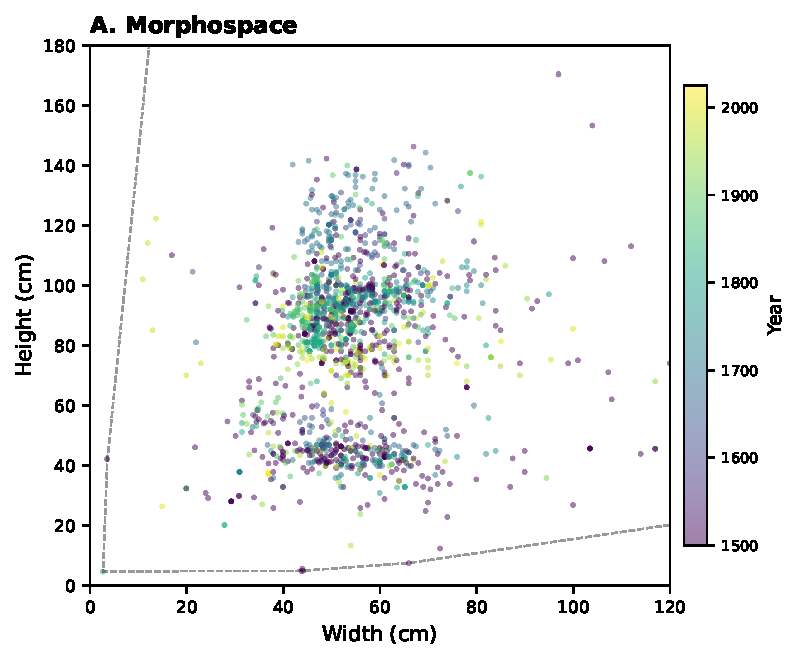
\includegraphics[width=\textwidth]{figures/fig-2-morphospace.pdf}
\end{minipage}%
\hfill
\begin{minipage}[t]{0.48\textwidth}
\centering
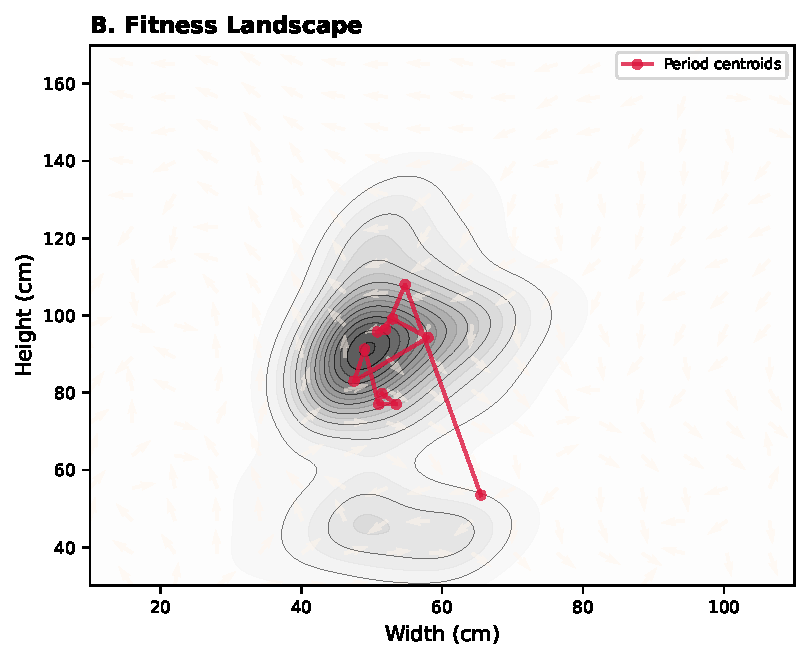
\includegraphics[width=\textwidth]{figures/fig-3-landscape.pdf}
\end{minipage}

\vspace{6pt}

% ── BOTTOM ROW: Structural panels ──
\begin{minipage}[t]{0.48\textwidth}
\centering
{\small\bfseries C.\enspace Multi-Scale Agency}\\[4pt]
\begin{tikzpicture}[
  scale=0.72, transform shape,
  cone/.style={draw=black!60, fill=black!4, thick},
  agent/.style={font=\scriptsize, text=black},
  label/.style={font=\tiny, text=black!70},
  >={Stealth[length=3pt]}
]
\draw[cone, fill=black!3] (-3.0, 0) -- (0, 4.8) -- (3.0, 0) -- cycle;
\node[agent, anchor=west] at (2.1, 0.3) {Market};
\node[label, anchor=west] at (2.1, 0.0) {decade};
\draw[cone, fill=black!5] (-2.2, 0) -- (0, 4.8) -- (2.2, 0) -- cycle;
\node[agent, anchor=west] at (1.5, 0.9) {Designer};
\node[label, anchor=west] at (1.5, 0.6) {month};
\draw[cone, fill=black!7] (-1.5, 0) -- (0, 4.8) -- (1.5, 0) -- cycle;
\node[agent, anchor=west] at (0.9, 1.6) {Tool};
\node[label, anchor=west] at (0.9, 1.3) {hour};
\draw[cone, fill=black!9] (-0.9, 0) -- (0, 4.8) -- (0.9, 0) -- cycle;
\node[agent, anchor=west] at (0.4, 2.4) {Material};
\node[label, anchor=west] at (0.4, 2.1) {minute};
\draw[cone, fill=black!12] (-0.35, 0) -- (0, 4.8) -- (0.35, 0) -- cycle;
\node[agent, anchor=east] at (-0.05, 3.2) {Cell};
\node[label, anchor=east] at (-0.05, 2.9) {ms};
\filldraw[black] (0, 4.8) circle (2pt);
\draw[decorate, decoration={brace, amplitude=4pt, mirror}, black!50]
  (-3.2, -0.1) -- (-3.2, 4.9) node[midway, left=6pt, font=\scriptsize, text=black!70, rotate=90, anchor=south] {cognitive cone $C(A)$};
\draw[<->, black!50] (-3.0, -0.5) -- (3.0, -0.5)
  node[midway, below, font=\scriptsize] {care $= \dim C(A)$};
\end{tikzpicture}
\end{minipage}%
\hfill
\begin{minipage}[t]{0.48\textwidth}
\centering
{\small\bfseries D.\enspace The Synthesis}\\[4pt]
\begin{tikzpicture}[
  scale=0.72, transform shape,
  box/.style={draw=black, rounded corners=3pt, minimum width=26mm, minimum height=8mm,
              font=\small, align=center, thick},
  pillar/.style={draw=#1, fill=#1!8, rounded corners=2pt, minimum width=22mm,
                 minimum height=6mm, font=\scriptsize, align=center},
  >={Stealth[length=3pt]}
]
\node[pillar=teal] (syn) at (-2.4, 4.2) {\textsc{Syntax}\\[-1pt]\tiny Stiny};
\node[pillar=orange!80!black] (log) at (0, 4.2) {\textsc{Logic}\\[-1pt]\tiny Hatchuel \& Weil};
\node[pillar=purple!70!black] (dyn) at (2.4, 4.2) {\textsc{Dynamics}\\[-1pt]\tiny Levin};
\node[box, minimum width=68mm, fill=black!5] (eq) at (0, 2.6)
  {$\mathrm{Form} = SG\!\left(\nabla_{C(A)}\, L(c,\,t)\right)$};
\node[box, fill=teal!8, draw=teal, minimum width=20mm] (sg) at (-2.4, 1.0) {$SG$\\[-2pt]\tiny grammar};
\node[box, fill=orange!8, draw=orange!80!black, minimum width=20mm] (lc) at (0, 1.0) {$L(c,t)$\\[-2pt]\tiny landscape};
\node[box, fill=purple!8, draw=purple!70!black, minimum width=20mm] (ca) at (2.4, 1.0) {$\nabla_{C(A)}$\\[-2pt]\tiny cone};
\node[box, fill=black!8, minimum width=46mm] (form) at (0, -0.4)
  {\textbf{Form} $x \in M(c)$};
\node[font=\small\itshape, text=black!80] (care) at (0, -1.4)
  {care $= \dim C(A)$};
\draw[->, thick, teal] (syn) -- (eq);
\draw[->, thick, orange!80!black] (log) -- (eq);
\draw[->, thick, purple!70!black] (dyn) -- (eq);
\draw[->, thick, teal] (eq) -- (sg);
\draw[->, thick, orange!80!black] (eq) -- (lc);
\draw[->, thick, purple!70!black] (eq) -- (ca);
\draw[->, thick] (sg) -- (form);
\draw[->, thick] (lc) -- (form);
\draw[->, thick] (ca) -- (form);
\draw[->, dashed, thick, black!50] (form.east) -- ++(1.0, 0) |- (lc.east)
  node[pos=0.25, right, font=\tiny, text=black!60] {$K$ expands};
\end{tikzpicture}
\end{minipage}

\caption{The architecture of \formlaere{}. \textbf{A}: 1,662 European chairs projected into morphospace (width $\times$ height); color encodes date. \textbf{B}: Fitness landscape as kernel density estimate with gradient vector field and period centroid trajectory (red). \textbf{C}: Nested cognitive cones across five competence scales; cone width corresponds to care dimensionality. \textbf{D}: The synthesis equation; three source traditions converge on the core equation; dashed arrow shows $K$-expansion feedback.}
\label{fig:architecture}
\end{figure*}


\begin{table*}[!t]
\centering
\caption{The seven main propositions of \formlaere{} with formal apparatus introduced by each.}
\label{tab:propositions}
\small
\begin{tabularx}{\textwidth}{@{}c >{\raggedright}p{0.28\textwidth} >{\raggedright}p{0.32\textwidth} >{\raggedright\arraybackslash}p{0.22\textwidth}@{}}
\toprule
\textbf{No.} & \textbf{Proposition} & \textbf{Formal apparatus} & \textbf{Source tradition} \\
\midrule
1 & The world of form is all that is the case & Morphospace, algebra, $C$-$K$ partition & Stiny; Hatchuel \& Weil \\[3pt]
2 & Not all positions are equally probable & Selection pressure, affordance & Gibson; Michl \\[3pt]
3 & The pressures produce a landscape & Fitness landscape, canalization & Wright; Waddington \\[3pt]
4 & The landscape is dynamic & Path dependence, adjacent possible & Arthur; Kauffman \\[3pt]
5 & Agents exist & $A := (g,d,\delta)$;\; care $= \dim C(A)$ & Levin; Doctor et al. \\[3pt]
6 & Form arises between agents & $\mathrm{Form} = SG(\nabla_{C(A)} L)$ & Synthesis \\[3pt]
7 & Form shows how far care reached & Ethical conclusion & --- \\
\bottomrule
\end{tabularx}
\end{table*}
